%==============================================================================
% Sjabloon poster bachproef
%==============================================================================
% Gebaseerd op document class `a0poster' door Gerlinde Kettl en Matthias Weiser
% Aangepast voor gebruik aan HOGENT door Jens Buysse en Bert Van Vreckem

\documentclass[a0,portrait]{hogent-poster}

% Info over de opleiding
\course{Bachelorproef}
\studyprogramme{toegepaste informatica}
\academicyear{2022-2023}
\institution{Hogeschool Gent, Valentin Vaerwyckweg 1, 9000 Gent}

% Info over de bachelorproef
\title{Sustainability in Continuous Integration en Deployment-processes}
\subtitle{A Comparative Analysis and Proof of Concept}
\author{Robbe Cherlet}
\email{robbe.cherlet@student.hogent.be}
\supervisor{Chantal Teerlinck}
\cosupervisor{Jan Delamper (Wolters Kluwer)}

% Indien ingevuld, wordt deze informatie toegevoegd aan het einde van de
% abstract. Zet in commentaar als je dit niet wilt.
\specialisation{Systeem- en Netwerkbeheer}
\keywords{Lambda-calculus, Scheme}
\projectrepo{https://github.com/BiggieBerto/Thesis/}

\begin{document}

\maketitle

\begin{abstract}
In the evolving landscape of software development, optimizing Continuous Integration and Deployment (CI/CD) processes has become critical for organizations aiming to maintain both efficiency and sustainability. This thesis addresses a concrete problem within a company, focusing on a detailed case study at Wolters Kluwer. The research is geared towards organizations looking to enhance their CI/CD workflows in a way that is both energy and cost-efficient, providing valuable insights for system administrators familiar with CI/CD concepts. By examining the environmental impact of current CI/CD practices, the study proposes practical solutions aimed at aligning these processes with sustainability principles.
  
\end{abstract}

\begin{multicols}{2} % This is how many columns your poster will be broken into, a portrait poster is generally split into 2 columns

\section{Introductie}

The drive to optimize Continuous Integration and Deployment (CI/CD) processes has become a significant concern in software development, particularly for organizations striving to balance efficiency with sustainability. This bachelor's thesis zeroes in on a practical case study within Wolters Kluwer, with the goal of assessing and improving the environmental footprint of their CI/CD practices.

This research is tailored for organizations interested in sustainable CI/CD optimization. By evaluating energy consumption and resource usage, the study aims to provide actionable recommendations to minimize environmental impact while maintaining high efficiency. The central research question explores how CI/CD practices can be refined to reduce their ecological footprint.

\section{Experimenten}
Through comprehensive data collection and best practice implementation, this study identifies significant opportunities for optimization. The findings illustrate that improving CI/CD workflows not only enhances operational efficiency but also contributes to environmental sustainability. The recommendations from this research promise to guide Wolters Kluwer—and potentially other organizations—towards more sustainable software development practices.

\section{Sectie met figuur}

% De {\LaTeX} figure-omgeving bepaalt zelf waar een afbeelding komt en dat is meestal niet op de plek in de tekst waar de figure-omgeving gedefinieerd wordt. Als je wilt forceren dat afbeeldingen toch in de flow van de tekst blijven, dan kan je dat zoals hieronder:

\begin{center}
  \captionsetup{type=figure}
  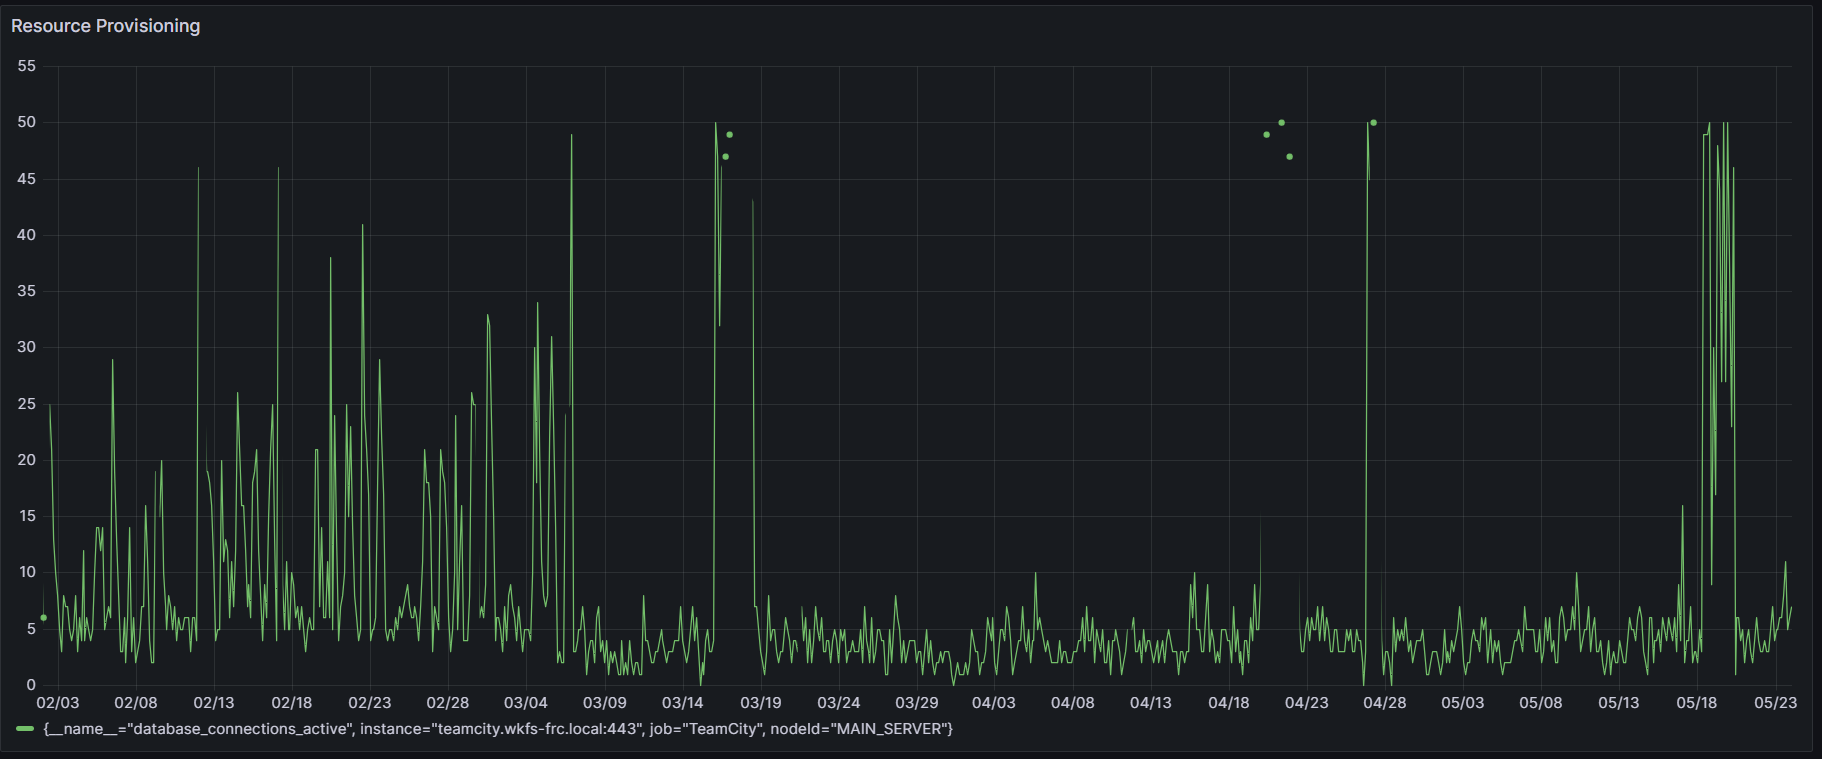
\includegraphics[width=1.0\linewidth]{graphics/DB connections.png}
  \captionof{figure}{Example of a result from the experiment.}
\end{center}

% Let er wel op dat dit tot problemen met bladschikking kan leiden.

\section{Conclusies}
This study contributes to the emerging field of sustainable software development by examining the environmental impact of CI/CD practices. The findings emphasize the importance of optimizing these processes to reduce energy consumption and resource waste. It was a challenge to implement these practices in a non-isolated environment, and it is clear that further research is needed to achieve more substantial reductions in environmental impact. Nevertheless, the insights gained from this research offer a valuable starting point for organizations looking to adopt greener CI/CD practices.

\section{Toekomstig onderzoek}
Future research should focus on refining the proposed recommendations and exploring additional strategies for optimizing CI/CD workflows. Investigating the impact of other processes on the CI/CD pipeline could provide further insights into how to reduce environmental impact. Additionally, conducting a comparative analysis of different CI/CD tools and practices in an isolated environment could help identify the most sustainable approaches for software development.

\end{multicols}
\end{document}